%!TEX TS-program = xelatex
\documentclass[]{friggeri-cv}
%\addbibresource{bibliography.bib}
%\usepackage{natbib}

\begin{document}
\header{}{个人简历}
       {}
% In the aside, each new line forces a line break
\begin{aside}
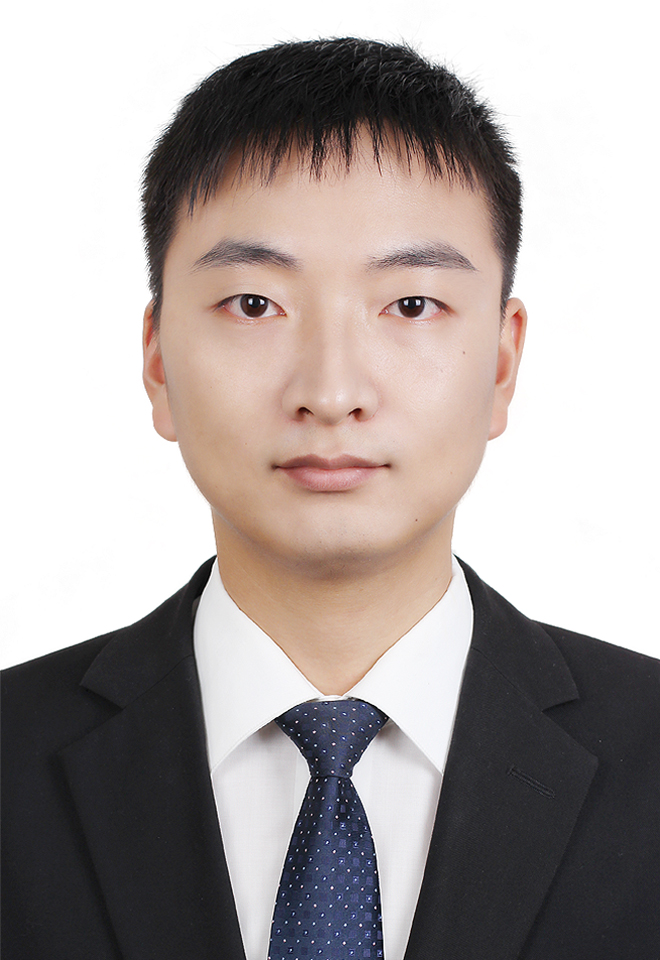
\includegraphics[width=4cm]{IMG_4827small.jpg}
  \section{个人简介}
   姓名:王腾飞 
   性别:男
   专业:计算地球物理
   1110701@tongji.edu.cn
   地址:上海市杨浦区
   四平路1239号
   电话:18817367538
  \section{外语等级}
  英语6级:522
  \section{编程开发技能}
	Unix/Linux
    C/C++
	MPI/OpenMP并行开发
    Shell/Python/Java
	SQL数据库
\end{aside}

\section{技能特长}
\large
熟悉Unix/Linux系统,有4年小型工作站/机群维护经验。精通C语言以及MPI,\\
OpenMP环境下的并行高性能计算算法设计,熟悉C++/Python/Java开发语言,\\
具有大型数据处理经验。熟悉常见算法及SQL数据库,具备良好的数学基础.\\

\section{教育经历}
\begin{entrylist}
  \entryTwo
    {2011-2017}
    {同济大学博士学位 \quad 专业:地球物理学}
%    {同济大学}
%    {专业:地球物理学}
  \entryTwo
    {2007-2011}
    {同济大学学士学位 \quad 专业:地球物理学}
%    {同济大学}
%    {专业:地球物理学}
\end{entrylist}

\section{研究经历}

\begin{entrylist}
  \entry
    {2010-2011}
    {方位各向异性介质局部角度域成像方法研究}
	{\emph{独立完成MPI算法程序设计并与导师合作发表英文SCI论文一篇}}
  \entry
    {2011-2013}
    {基于深度域角道集的层析速度模型建立}
    {\emph{移植大型稀疏矩阵求解的开源软件包并利用该软件实现\\
	地球物理问题中稀疏矩阵的MPI/OpenMP并行求解}}
  \entry
    {2013-2015}
    {基于模式解耦的弹性波全波形反演方法}
    {\emph{
		完成算法设计,并利用MPI+OpenMP的混合编程方式解决该算法
		中大规模数据处理方面的内存,任务平衡等实际问题,并以第一\\
		作者发表英文SCI论文一篇
	}}
  \entry
    {2015--}
    {基于模式解耦的弹性波反射波全波形反演方法}
	{\emph{
		移植 Java和Python平台的音频、视频识别开源算法到已有算法中,\\
		利用该领域中的动态时间归整算法来对地球物理数据进行模式识\\
		别,从而实现对反射波数据的拟合,该课题的论文正在撰写中
	}}
\end{entrylist}

\section{实践经历}
\begin{entrylist}
  \entry
    {2011-2012}
    {中石化南京物探研究院}
	{\emph{
		参与导师与该研究院的合作项目并负责完成算法在其科研平台上\\
		的测试与移植,并完成了算法的部分加速优化。
	}}
  \entry
    {2012-2014}
    {中石油川庆钻探地球物理勘探公司}
	{\emph{
		参与导师与该单位的合作项目并负责深度域建模算法在该单位独\\
		立开发软件上的移植工作。
	}}
\end{entrylist}
\section{获得荣誉}
\begin{entrylist}
  \entryTwo
    {2011}
    {刘光鼎地球物理奖学金}
  \entryTwo
    {2012}
	{研究生国家奖学金}
  \entryTwo
    {2013}
    {同济大学地球物理奖学金}
\par\vspace{\parskip}
%\vspace{3cm}
\end{entrylist}

\section{发表论文}
\begin{entrylist}
  \entry
    {2012}
	{Geophysics: Azimuth-preserved local angle-domain prestack \\
	time migration in isotropic	vertical transversely isotropic\\
	and azimuthally anisotropic media}
	{\emph{程玖兵,王腾飞,王晨龙,耿建华}}
  \entry
    {2016}
	{Geophysics: Elastic full waveform inversion based on mode\\
		decomposition: The approach and	mechanism
	}
	{\emph{王腾飞,程玖兵(审稿中)}}
\end{entrylist}

\section{国际交流}
\begin{entrylist}
  \entry
    {2016}
    {沙特国王科技大学3个月访问学者}
	{\emph{
		导师国际合作项目的进展与下一步合作工作规划的交流
	}}
  \entry
    {2016}
    {欧洲勘探地球物理联合会年会}
	{\emph{会议口头报告: Comparison between mode decomposition based and Gaussian Newton methods in
		elastic full waveform inversion
	}}
  \entry
    {2015}
    {欧洲勘探地球物理联合会年会}
	{\emph{会议口头报告: 
		Elastic wave mode decoupling for full waveform inversion
	}}
  \entry
    {2012}
    {全球勘探地球物理学家年会}
	{\emph{会议口头报告: Pure mode modeling and reverse-time migration of P-wave in
		HTI and orthorhombic media
	}}
\end{entrylist}
\end{document}
